\section{Grundlagen}
\subsection{Wichtige Formeln}
    \renewcommand{\arraystretch}{2}
    \begin{longtable}{| p{.25\textwidth} | p{.40\textwidth} | p{.30\textwidth} |}
        \firsthline
        \textbf{Elektrische Kraft} \newline
        \tabbild[width=3.5cm]{images/ElKraft.png} \newline {\tiny Die Kraftwirkung des geladenen Körpers (Q) auf eine elektrische Probeladung (q)}&
        \begin{equation*}\vec{F_e}(r) = \dfrac{1}{2\pi\epsilon}\cdot\dfrac{Q\cdot q}{r}\cdot\vec{r_0}\end{equation*}
        \begin{equation*}F_e(r) = \dfrac{\pi\cdot\epsilon\cdot U^2}{2\cdot r\cdot\left(ln\dfrac{r-R_1}{R_1}\right)^2}\end{equation*} & \newline
        [${F_e}$] = $\dfrac{N}{m}$\newline \newline 
        $\epsilon=\epsilon_0\cdot\epsilon_r\newline
        \widehat{=}\,${\small dielektrische Permittivität}\newline 
        $\epsilon_0 = 8.8542 \cdot 10^{-12}$ $\left[\dfrac{As}{Vm}\right]$ \newline
        $\vec{r_0}=\dfrac{\vec{r}}{|\vec{r}|}\,\widehat{=}$ Einheitsvektor \newline  
        Q, q$\,\widehat{=}\,$Linienladungsdichte$\,\left[\dfrac{C}{m}\right]$ 
        \\ \hline
        
        \textbf{Magnetische Kraft} \newline
        \tabbild[width=3.5cm]{images/magnetischeKraft.png}   &	
        \begin{equation*}\vec{F_m}(r) = \dfrac{\mu}{2\pi}\cdot\dfrac{I\cdot i}{r}\cdot\vec{r_0} = \mu\cdot i\cdot \vec{l_0}\times\vec{H}\end{equation*} 
        \begin{equation*}F_m(r) = \dfrac{\mu\cdot I^2}{2\cdot\pi\cdot r}\end{equation*} 
        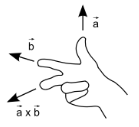
\includegraphics[width=3cm]{images/vektorprodukt.png}	& \newline
        $\mu =\mu_0\cdot\mu_r$\newline $\widehat{=}$ magnetische Permeabilität\newline 
        $\mu_0$ = $4\pi\cdot 10^{-7} \,\left[\dfrac{N}{A^2}\right]=\left[\dfrac{Vs}{Am}\right]$ \newline \newline
        $\vec{r_0}=\dfrac{\vec{r}}{|\vec{r}|}\,\widehat{=}$ Einheitsvektor \newline \newline 
        I, i $\widehat{=}$ elektrische Ströme 	\newline \newline 
        $[F_m]$ = $\dfrac{N}{m}$
        \\ \hline
    \end{longtable}  
    
    \begin{minipage}{7cm}
        \textbf{BSP:}\newline
         .\hspace{3.5cm}\tabbild[width=8cm]{images/BspVergleich}
    \end{minipage}
    \begin{multicols}{2}
        \begin{minipage}{\linewidth}
           \textbf{Elektrische Kraft vs.}\newline
            \begin{equation*}
            F_e(r) = \dfrac{\pi\cdot\epsilon\cdot U^2}{2\cdot r\cdot\left(ln\dfrac{r-R_1}{R_1}\right)^2} = 2.88\cdot 10^{-11} \quad \left[\dfrac{N}{m}\right]
            \end{equation*}
        \end{minipage}

        \begin{minipage}{\linewidth}
            \textbf{Magnetische Kraft}\newline
            \begin{equation*}
             F_m = \dfrac{\mu_0\cdot I^2}{2\cdot\pi\cdot r} = 2.00 \cdot 10^{-6} \quad\left[\dfrac{N}{m}\right]
            \end{equation*}
        \end{minipage}        
    \end{multicols}
    
    \begin{minipage}{\linewidth}
        \vspace{0.5cm}
        Die magnetische Kraft pro Länge \& Strom ist $7 \cdot 10^4$ grösser als jene der elektrische Kraft.\newline Daher basieren \textbf{alle} elektrischen Maschinen auf der magnetischen Kraft.\newline 
    \end{minipage}
    
    \begin{minipage}{\linewidth}  
        \renewcommand{\arraystretch}{1} 
        \begin{tabular}{|p{0.4\linewidth}|p{0.25\linewidth}|p{5cm}|}
            \hline
            \textbf{Exkurs Vektorprodukt}\newline             
            \[ \vec{a}\times\vec{b}=|\vec{a}|\cdot|\vec{b}|\cdot sin(\theta) \] 
            $ Wenn \; \vec{a}\bot\vec{b} $ \newline
           \[  \vec{a}\times\vec{b}=|\vec{a}|\cdot|\vec{b}| \] & \vspace{0.3cm}
           $ \theta$ = Zwischenwinkel in \textdegree &\vspace{0.8cm}
           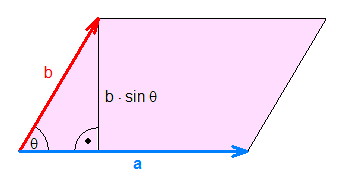
\includegraphics[width=5cm]{images/Kreuzprodukt}
           \\
            \hline 
        \end{tabular}                 
    \end{minipage}
    

    \clearpage
    \subsubsection{Elektrische Kraft}    
    \begin{longtable}{| p{.25\textwidth} | p{.40\textwidth} | p{.30\textwidth} |}    
        \firsthline
        \textbf{Elektrisches Feld} \newline \newline
        \tabbild[width=4cm]{images/elektrischesFeld.png} &
        \begin{equation*}\vec{E} = \dfrac{\vec{F_e}}{q} = \dfrac{1}{2\pi\epsilon}\cdot\dfrac{Q}{r}\cdot\vec{r_0}\end{equation*} 
        \begin{equation*}\vec{E} = \dfrac{1}{2\pi\epsilon}\cdot\dfrac{Q}{r}\cdot\vec{r_0}\end{equation*} & 
        \begin{equation*}[E] = \dfrac{V}{m}\end{equation*} 									
        \\ \hline
        
        \textbf{Elektrisches Potential}  &
        \begin{equation*}\varphi_A = \int_{A}^{Bezugspunkt}\vec{E}\cdot\vec{dl}	\end{equation*}	& 
        \begin{equation*}[\varphi_A] = V\end{equation*} 
        \\ \hline
        
        \textbf{Elektrische Spannung}   &
        \begin{equation*}U_{AB} = \int\limits_{A}^{B}\vec{E}\cdot\vec{dl} = \varphi_A - \varphi_B\end{equation*}  & 
        \begin{equation*}[U] = V \end{equation*}  
        \\ \hline
              
        \textbf{Elektrischer Strom} 	    &  
        \begin{equation*}I = \dfrac{dQ}{dt} = \dot{Q}	\end{equation*} &  
        \begin{equation*}[I] = A\end{equation*} 
        \\ \hline    
    \end{longtable}   
    \clearpage
    \subsubsection{Magnetische Kraft}     
    \begin{longtable}{| p{.25\textwidth} | p{.40\textwidth} | p{.30\textwidth} |}  
        \firsthline		
        \textbf{Magnetische Feldstärke} \newline \newline
        \tabbild[width=4cm]{images/magnetischesFeld.png} &
        \begin{equation*}\vec{H} = \dfrac{I}{2\pi}\cdot\dfrac{\vec{L_0}\times\vec{r_0}}{r} \end{equation*}  \tabbild[width=4cm]{images/MagnetischeFeldstaerke} & 
        \newline [H] = $\dfrac{A}{m}$ \newline \newline
        $\vec{L_0},\vec{l_0}$ $\widehat{=}$ Einheitsvektoren der Stromleiter
		\newline \newline
        $\vec{r_0}=\dfrac{\vec{r}}{|\vec{r}|}\,\widehat{=}$ Einheitsvektor
        \\ \hline
        
        \textbf{Magnetische Flussdichte}  &
        \begin{equation*}\vec{B} = \mu\cdot\vec{H} = \mu_0\cdot\mu_r\cdot\vec{H}\end{equation*} &  
        \begin{equation*}[B] = T=\dfrac{Vs}{m^2}\end{equation*} \[ \mu_0$ = $4\pi\cdot 10^{-7} \,\left[\dfrac{N}{A^2}\right]=\left[\dfrac{Vs}{Am}\right]\]
        \\ \hline
        
        \textbf{Magnetische Fluss} \newline
        \tabbild[width=3.5cm]{images/magnetischeFluss} & 
        \begin{equation*}\phi = \iint\limits_{(A)}\vec{B}\cdot\vec{dA}\end{equation*} &  
        \begin{equation*}[\phi] = Vs = Wb\end{equation*}
        \\ \hline
        
        \textbf{Verkettete Fluss}\newline 
        \tabbild[width=4cm]{images/Verkettetefluss}		 &
        \begin{equation*}\psi = N\cdot\phi\end{equation*}
        \begin{equation*}\psi = L\cdot I\end{equation*}
        \centering\textbf{meistens} 
        \begin{equation*}\psi(t) = N\cdot\iint\limits_{(A)}\vec{B}\cdot\vec{dA}=N\cdot B \cdot A \cdot cos\left(\omega t\right)\end{equation*} & 
        \begin{equation*}[\psi] = Vs = Wb\end{equation*}
        \\ \hline
        
        \textbf{Induzierte Spannung} 	 &
        \begin{equation*}U_{ind} = -\dfrac{d\psi}{dt}=-N\dfrac{d\phi}{dt}\end{equation*}			
        \centering\textbf{meistens} 
        \begin{equation*}U_{ind} = -\dfrac{d\psi}{dt}=\omega\cdot N\cdot B\cdot A\cdot sin\left(\omega t\right)\end{equation*}  &
        \\ \hline
        
        \textbf{Magnetische Durchflutung} \newline \newline
        \tabbild[width=4cm]{images/Durchflutungssatz.png}  &
        \begin{equation*}	 \Theta = \sum\limits_{k=1}^{n}I_k = \oint\limits_{(C)}\vec{H}\cdot\vec{dl}\end{equation*}  
        \centering\textbf{Beispiel:}\
        \begin{equation*}	\oint\limits_{(C)}\vec{H}\cdot\vec{dl} = \int \limits_{P_1}^{P_2}\vec{H}\cdot\vec{dl} + \int \limits_{P_2}^{P_3}\vec{H}\cdot\vec{dl}	+ ... + \int \limits_{P_{m-1}}^{P_m}\vec{H}\cdot\vec{dl}\end{equation*}				&
        \begin{equation*}[\Theta] = A\end{equation*} 
        \\ \hline
        
        \textbf{Magnetische Spannung}	 & 
        \begin{equation*}V_m = \int\limits_{A}^{B}\vec{H}\cdot\vec{dl} \approx H_{Luft}\cdot l_{Luft} = V_{mLuft} \end{equation*}											
        & \begin{equation*}[V_m] = A\end{equation*} 
        $ \approx $ Nur wenn der Kern \textbf{nicht} in \qquad Sättigung
        \\ \hline 
        \textbf{Magnetkreis}	\newline
        \tabbild[width=4cm]{images/magnetkreis.png}  &
        \begin{equation*}\oint\limits_{(C)}\vec{H}\cdot\vec{dl} \approx H\cdot L = N\cdot I\end{equation*}  
        \begin{equation*}\Rightarrow H = \dfrac{N\cdot I}{L}\end{equation*} 
        \begin{equation*}\Rightarrow B = \mu_0\cdot\dfrac{N\cdot I}{L}\end{equation*} &    
        falls L $>>$ R und \newline 
        das Feld in der Spule \textbf{homogen} ist \newline \newline \textcolor{red}{\danger \, L ist hier die Länge!}
        \\ \hline
        
        \textbf{Reluktanzkraft} \newline
        \tabbild[width=3cm]{images/reluktanzkraft.png} &
        \vspace{-0.5cm}
        \begin{equation*}F_R = -\dfrac{\partial W_m}{\partial\delta}=\frac{F_1}{2}= \mu_0\cdot\dfrac{N^2\cdot I^2\cdot A_{Fe}}{4\cdot\delta^2}\end{equation*}
        \[F_1 = \mu_0\cdot\dfrac{H^2\cdot A_{Fe}}{2}= \mu_0 \cdot \frac{N^2\cdot I^2 \cdot A_{Fe}}{\delta^2 \cdot 2} \] & 
        wobei $A_{Fe}$ die magnetisch \newline wirksame Fläche des Luftspalts ist. \newline
        $ F_1 $= Kraft bei 1nem Luftspalt\newline
        $ F_R $= Kraft beider Luftspalte\newline
        $ \delta $= Länge 1nes Luftspaltes
        \\ \hline
        \textbf{Magnetische Energie} & 
        $W_m = \dfrac{1}{2}\cdot H_\delta\cdot B_\delta\cdot2\cdot A_{Fe}\cdot\delta = \mu_0\cdot \dfrac{I^2\cdot N^2}{4\cdot\delta}\cdot A_{Fe}$
        \newline\newline $W_m = \dfrac{1}{2}\cdot\iiint\limits_{(V)}\vec{B}\cdot\vec{H}\cdot dV = \dfrac{1}{2}\cdot\iiint\limits_{(V)}\dfrac{1}{\mu}\cdot B^2\cdot dV$&wobei $A_{Fe}\cdot\delta$ dem Volumen des Luftspalts entspricht. \\
        \hline
		\textbf{Magnetischer Widerstand} \newline \tabbild[width=3cm]{images/MagnetischeWiderstand} & 
        \[ R_m = \dfrac{V_m}{\phi}\] \newline wenn $\vec{A} \perp \vec{\phi} :$ \newline 
        \[R_m = \dfrac{H_0\cdot l}{B_0\cdot A} = \dfrac{l}{\mu_0\cdot A}\] & 
        \[[R_m] = \dfrac{A}{Vs} \] \\
		\hline
    \end{longtable}
    \clearpage
